\documentclass{report}

% ----------------------------------------------------------------------------
% Preamble
% ----------------------------------------------------------------------------

% These are some lazy packages to get a good looking page layout
\usepackage{fullpage}
\usepackage[parfill]{parskip}

\usepackage{setspace}
\onehalfspacing

% A package to include graphics files (jpg, png, eps, pdf etc...)
\usepackage{graphicx}

% Some basic packages that are almost standad
\usepackage{amssymb}

% Package to be able to draw tikz images
\usepackage{tikz}
\usetikzlibrary{calc}

% Package to get hyperrlinks
\usepackage{hyperref}

% Package to be able to compile standalone tikz packages
\usepackage{standalone}

% A package that changes the header.

% A package that gives more control for bibliographies than the default
\usepackage[backend=biber, backref=true, firstinits=true, url=true, isbn=true]{biblatex}
\addbibresource{bibliography.bib}

% A package to generate latin. You do not need this: I am just using it to get
% random text.
\usepackage{lipsum}

% ----------------------------------------------------------------------------
% The actual report
% ----------------------------------------------------------------------------

\begin{document}
    \begin{titlepage}
    \begin{center}
        \vspace*{5cm}

        \textbf{Thesis Title}

        \vspace{0.5cm}
        Thesis Subtitle

        \vspace{1.5cm}

        \textbf{James Campbell}

        \vfill

        B.Sc. Final Year Dissertation\\

        \vspace{0.5cm}
        Cardiff School of Mathematics

        \vspace{1.5cm}

        
\includegraphics[width=0.8\textwidth]{../img/universitylogo.eps}


    \end{center}
\end{titlepage}

    \Huge{\textbf{Acknowledgments}}

\normalsize

\vspace{1.5cm}

\lipsum[1-4]


    \tableofcontents
    \listoffigures

    % The actual content:
    \chapter{Introduction}\label{cha:introduction}

\section{Introduction}

There is this data that is pretty awesome, I'm going to plot it and show it to
you in sections~\ref{sec:the_data} and~\ref{sec:the_distribution_of_the_data}.

\lipsum

\section{The data}\label{sec:the_data}

In Figure~\ref{fig:the_data} we see data that was generated using
(\ref{equ:random_data}):

\begin{equation}
    x \in \{x \in \mathbb{Z}| 1 \leq x \leq 1999\}
\end{equation}

\begin{equation}
    y = 2(1 + \epsilon) x + 5\label{equ:random_data}
\end{equation}

where \(\epsilon\in(-0.5, 0.5)\) is a random number.

\begin{figure}[!hbtp]
    \begin{center}
        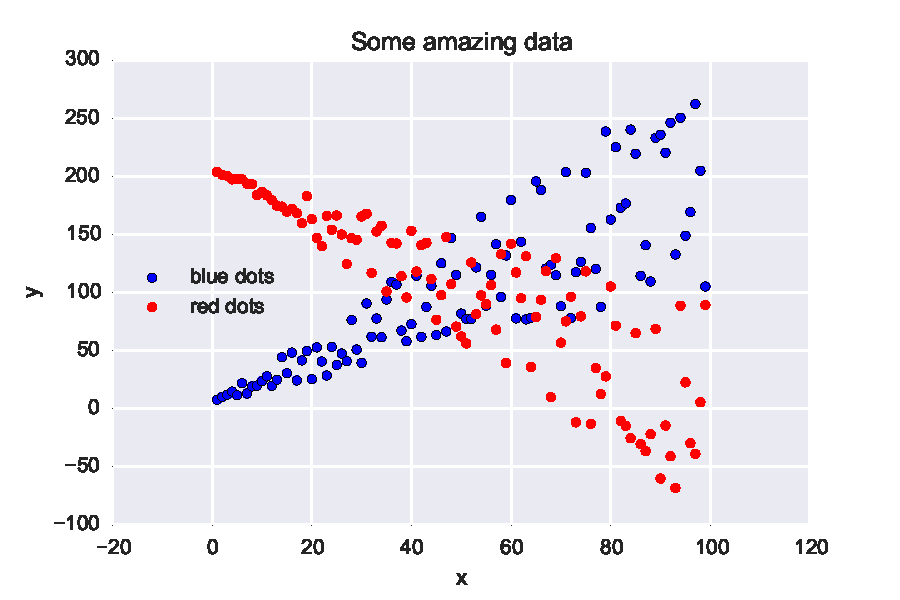
\includegraphics[width=.6\textwidth]{../img/plot1.pdf}
        \caption{The great data}\label{fig:the_data}
    \end{center}
\end{figure}

\section{The distribution of the data}\label{sec:the_distribution_of_the_data}

Figure shows the distribution of the data.

\begin{figure}[!hbtp]
    \begin{center}
        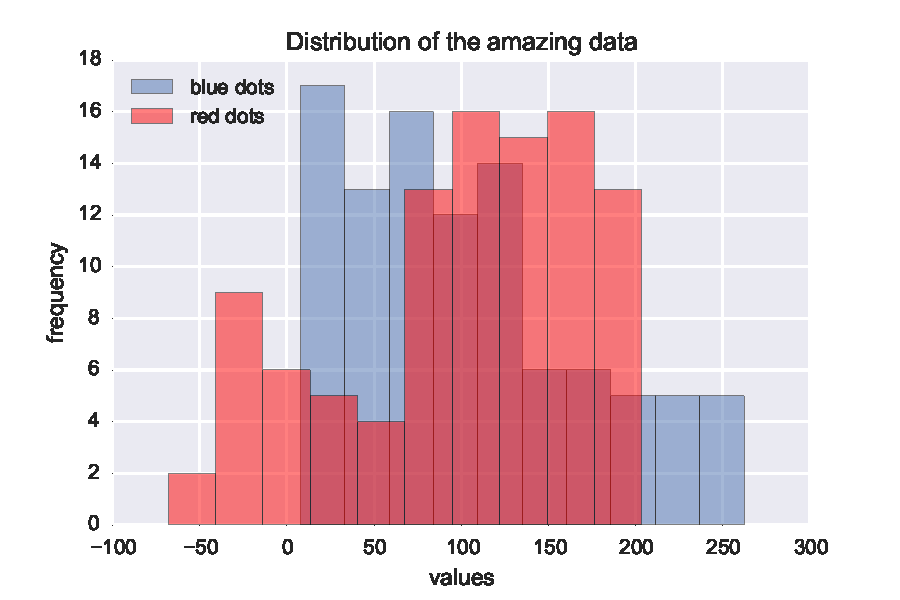
\includegraphics[width=.6\textwidth]{../img/plot2.pdf}
        \caption{The distribution of the great data}\label{fig:the_distribution_of_the_data}
    \end{center}
\end{figure}

\lipsum

\section{Conclusion}\label{sec:conclusion}

This chapter was amazing, here is a reference to a paper~\cite{Gillard2014}.


    \chapter{Awesome theorems and stuff}\label{cha:awesome_theorems_and_stuff}

\section{Introduction}

Note that I can refer to other chapters: see Chapter~\ref{cha:introduction} and
even specific equations in each chapter, this is an
equation~(\ref{equ:random_data}).

\lipsum

    %!TEX root = ../main.tex

\chapter{Conclusion}\label{cha:conclusion}

\section{Introduction}

This chapter will just show you a picture drawn in tikz shown in
Figure~\ref{fig:markov_chain}.

\begin{figure}[!hbtp]
    \begin{center}
        \includestandalone{../img/markov_chain}
        \caption{A Markov chain}\label{fig:markov_chain}
    \end{center}
\end{figure}

\section{Conclusion}

The end.

\lipsum


    % The bibliography:
    \printbibliography
\end{document}
